\documentclass[10pt,final]{beamer} %,hyperref={pdfpagelabels=false},draft,handout,handout
\input{rm3.sty}
%\let\Tiny=\tiny

%\includeonlyframes{current,current1,current2}

\lecture[1]{La matematica per la cooperazione}{Artin Conjecture}
\date{October 23-24, 2013}


\title[La matematica per la cooperazione]{\insertlecture}
\subtitle{\ }

\begin{document}

\begin{frame}
\titlepage
\end{frame}


\section{CIMPA}

\begin{frame}\frametitle{Centro Interuniversitario per la Matematica Pura e Applicata}
\framesubtitle{ (CIMPA)\ http://www.cimpa-icpam.org}

\begin{itemize}
 \item C.I.M.P.A (\textsc{Centro Internazionale di Matematica Pura ed Applicata});
\item dagli anni 90 \textbf{centro UNESCO di seconda categoria};
\item organizzazione internazionale senza scopo di lucro fondata a Nizza (Francia) nel 1978;
\item \textbf{scopo:} 
\textit{Promuovere la cooperazione internazionale nel campo dell'istruzione superiore 
e della ricerca in \textbf{matematica} e materie affini, in particolare dell'informatica a beneficio dei paesi in via di sviluppo.}
\end{itemize}
\hfill\ \includegraphics[width=1.5cm]{logo-cimpa.jpeg}
\end{frame}
\section{Scuole di Ricerca}

\begin{frame}
\frametitle{Centro Interuniversitario per la Matematica Pura e Applicata (CIMPA)}
\framesubtitle{Le scuole di ricerca CIMPA}

\begin{columns}[c]
\begin{column}{4.5cm}

\large{\ \ 2014}
\begin{itemize}
 \item Cile, Colombia, Messico
\item Costa d'Avorio, Senegal, Benin, Marocco,
Algeria
\item Palestina, Libano, Turchia
\item Pakistan, Nepal, Kurdistan Iracheno, India
\item Indonesia, Filippine, Laos
\end{itemize}
\end{column}
\begin{column}{5.5cm}
\includegraphics[width=5.5cm]{Poster2014-3.jpg}
\end{column}
\end{columns}
\end{frame}

\section{Roma Tre e CIMPA} 
\begin{frame}
\frametitle{La collaborazione tra Roma Tre e CIMPA per la scuole di Ricerca}

\begin{itemize}
 \item (2010) \textbf{Nepal:}\\
Number Theory in Cryptography and Its Applications\\
\textsl{Kathmandu University, Dhulikhel}
\item (2011) \textbf{Mali:}\\ 
Th\'eorie des nombres et algorithmique\\
\textsl{Universit\'e de Bamako}
 \item (2013) \textbf{Filippine}: in collaborazione di ICTP\\ 
Algebraic Curves over finite fields and applications\\
\textsl{University of the Philippines Diliman}
\item (2013) \textbf{Mongolia:}\\
Hypergeometric Functions and Representation Theory\\
\textsl{National University of Mongolia, Ulaanbaatar}
\item (2014) \textbf{Benin}: in collaborazione di ICTP\\ 
Algebraic Number Theory and applications\\
\textsl{Institute of mathematics and physical Sciences, Dangbo}
 \item (2016) \textbf{Albania:} ??\\
\textsl{Universiteti i Vlor\"e}
\end{itemize}
\end{frame}

\section{Altro}
\begin{frame}
\frametitle{Altre collaborazioni}
\framesubtitle{Teoria dei Numeri}
\begin{itemize}
\item (2009--) \textbf{Nepal:}\\
\textsl{National School on Number Theory and Cryptography}, \\
Kathmandu University, \textbf{Dhulikhel}
\item (2013--) \textbf{Iraq:}\\
\textsl{Second International Conference in Mathematics and Applications,}\\
University of Barsah, \textbf{Bassora}
\item (2013) \textbf{Bangladesh:}\\
\textsl{$18^{\text{th}}$ Mathematical Conference}\\
Independent University, Bangladesh, \textbf{Dhaka}
 \item (2015--) \textbf{Albania:}\\
\textsl{Scuola estiva di Teoria dei Numeri (??)}\\
\textbf{Vlor\"e}
\end{itemize}
\end{frame}

\section{Foto}
\begin{frame}
\frametitle{Foto Ricordo:}
\includegraphics[width=4.85cm]{Kathmandu.jpg}\ 
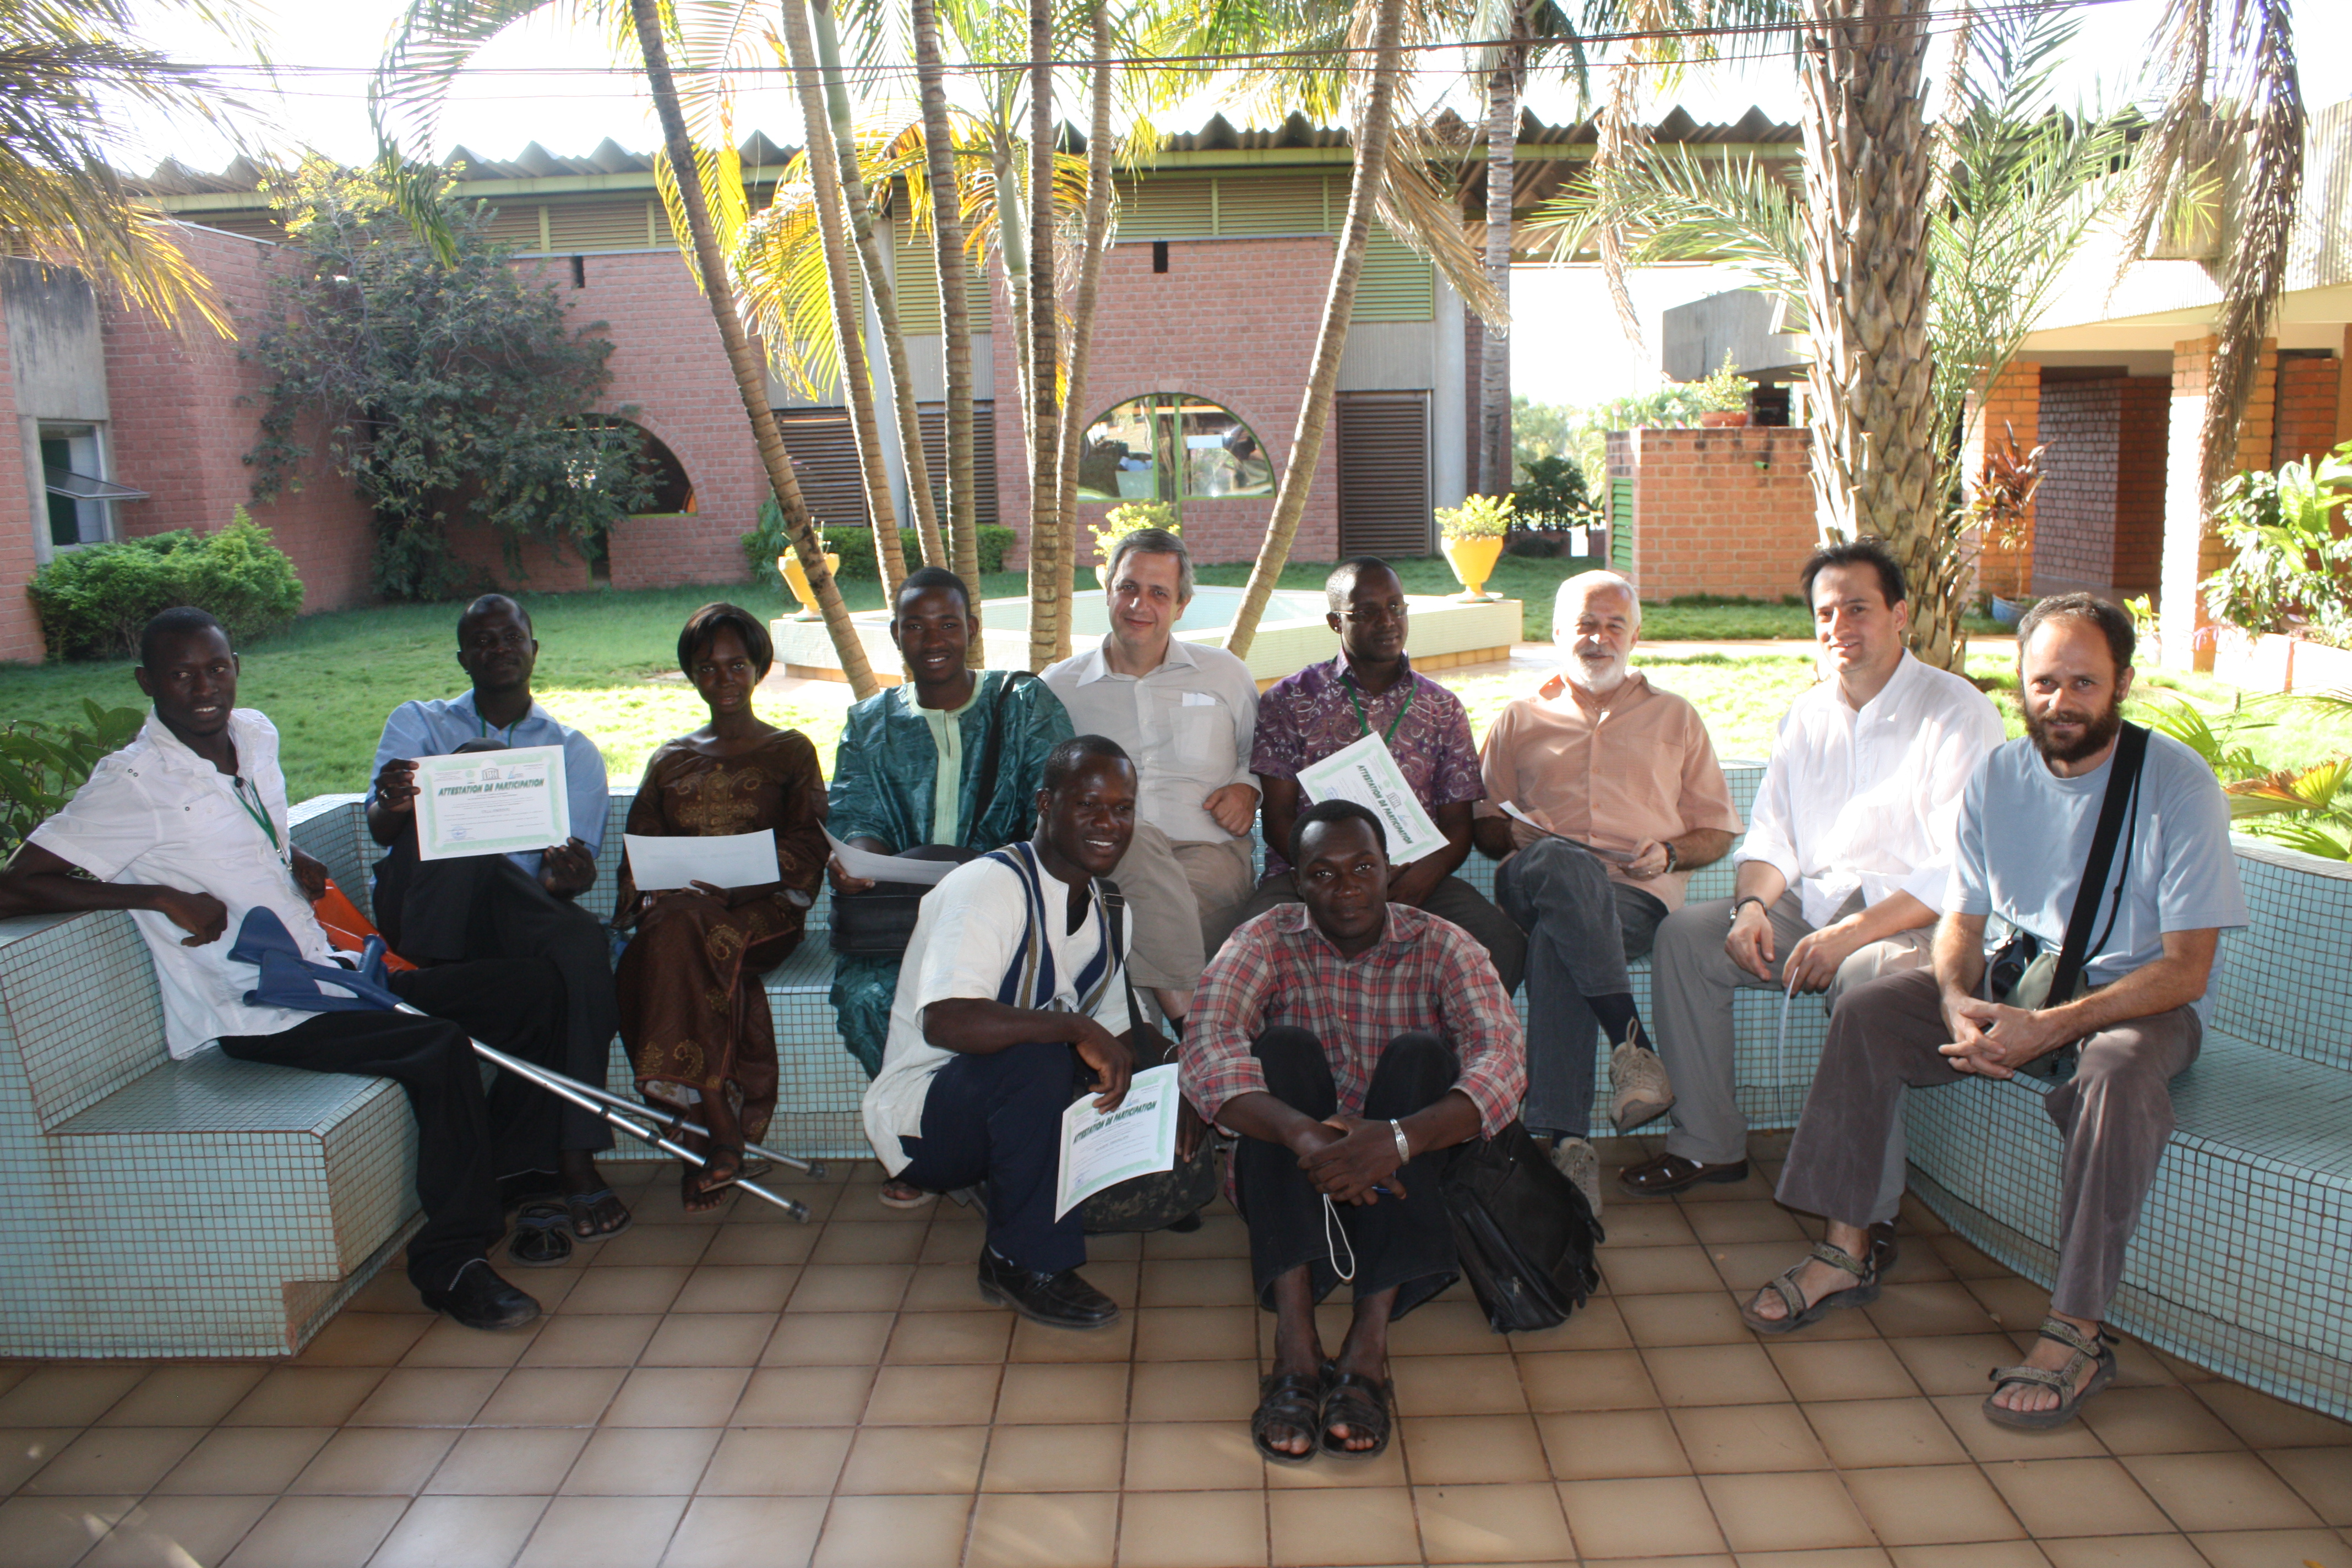
\includegraphics[width=4.85cm]{Mali2010355.jpg}\\
Kathmandu \hfill Bamako\bigskip

\includegraphics[width=4.85cm]{CIMG0516.JPG} \
\includegraphics[width=4.85cm]{2013-10-23-141.jpg}\\
Manila \hfill Bassora

\end{frame}
\end{document}

